\section { Michal Zieba}
\label{ sec:Michal Zieba}

\textbf{Wzór na długość przeciwprostokatnej w trojkącie prostokątnym, gdzie a i b to przyprostokątne:}
\begin{center}
$c =\sqrt{a^{2}+b^{2}}$



    a tutaj kotek.


\begin{figure}[htbp]
    \centering
    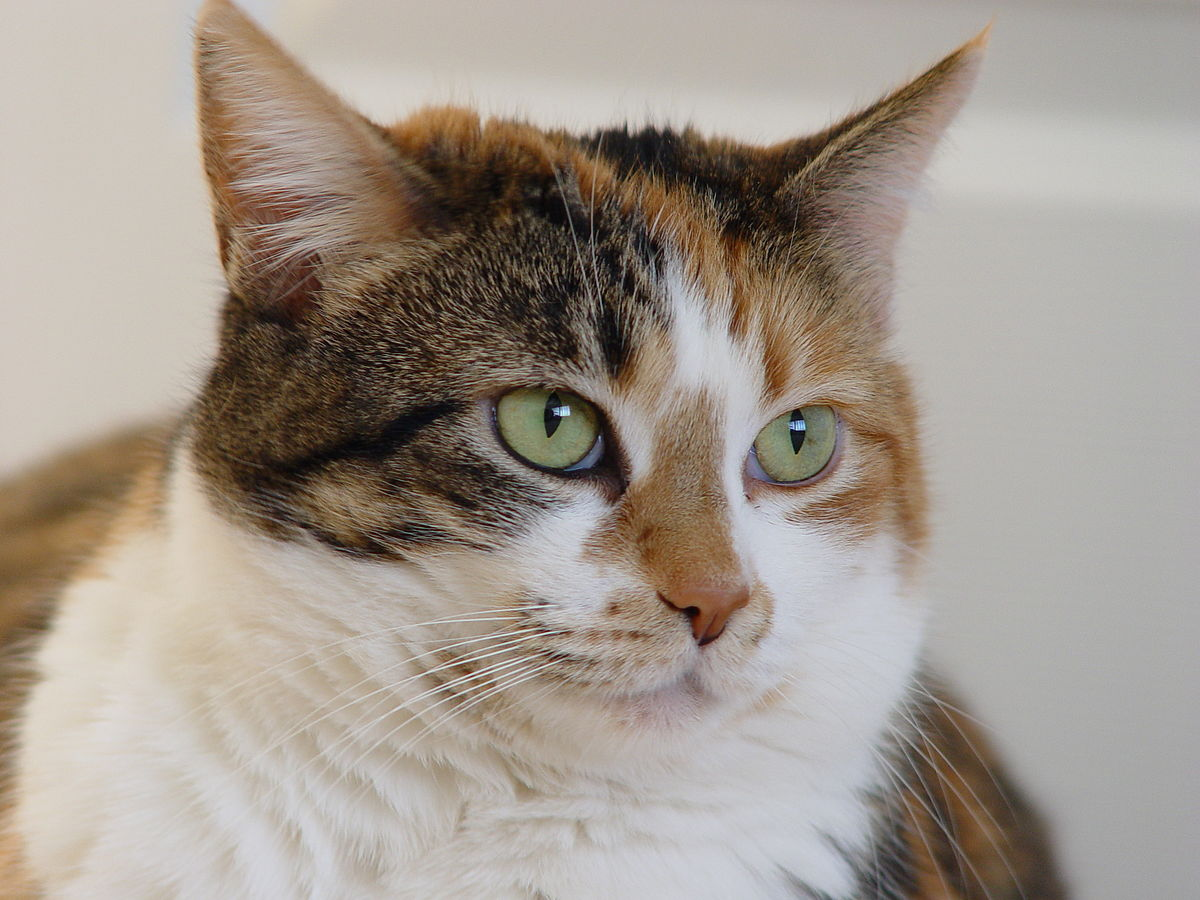
\includegraphics[width=0.3\textwidth]{pictures/cat.jpg}
    \caption{kotek.}
    \label{fig:cat}
\end{figure}


\break
\subsection{Listy}
{ \textbf{ Top 5 ludzi}}
\textit{
\begin{enumerate}
        \item Każdy
        \item Człowiek
        \item Jest
        \item Równy
        \item Mariusz Pudzianowski
\end{enumerate}
}
\begin {table}[htbp]
\label{tab:Przykladowa tabelka}
\begin{tabular}{|l|l|l|l|l|}
\hline
num & x & y & z & w \\ \hline
x   & 3 & 4 & 5 & 1 \\ \hline
y   & 4 & 5 & 1 & 2 \\ \hline
z   & 5 & 1 & 2 & 3 \\ \hline
\end{tabular}
\end{table}
 
\textbf{Lista Rzeczy}
\begin{itemize}
    \item Chleb
    \item toster
    \item wanna
\end{itemize}
\subsection{Teksty}
\begin{center}
    "Lorem ipsum dolor sit amet, consectetur adipiscing elit, sed do eiusmod tempor incididunt ut labore et dolore magna aliqua. Ut 
    \begin{center}
            enim ad minim veniam, quis nostrud exercitation ullamco laboris nisi ut aliquip ex ea commodo consequat. Duis aute irure dolor 
    in reprehenderit in voluptate velit esse cillum dolore eu fugiat nulla pariatur. Excepteur sint occaecat cupidatat non proident, sunt in culpa qui officia deserunt mollit anim id est laborum."
    \end{center}
\end{center}
\end{center}